\documentclass[10pt,conference,a4paper]{IEEEtran}
\usepackage[utf8]{inputenc} 
\usepackage{textcomp}
%%**************************************************
%% WICHTIG: Je nach Sprache des Textes die 
%% folgende Zeile anpassen
\usepackage[ngerman]{babel} % ngerman
%%**************************************************
\usepackage{xspace}
\usepackage[nocompress]{cite}
\usepackage[bottom]{footmisc}
\usepackage{booktabs}
\usepackage[pdftex]{graphicx}
%\usepackage[caption=false,font=footnotesize,labelfont=sf,textfont=sf]{subfig}
\usepackage{stfloats}
\usepackage{xurl}
\usepackage{listings}

\urlstyle{tt}


% correct bad hyphenation here
\hyphenation{op-tical net-works semi-conduc-tor}


\begin{document}
% paper title
\title{Docker, Möglichkeiten und Fallstricke der Containerisierung von Legacy Software}

% author names and affiliations
\author{%
	\IEEEauthorblockN{Andreas Scheuer}%
	\IEEEauthorblockA{%
		htw saar -- Hochschule für Technik und Wirtschaft des Saarlandes \\ %
		Seminar ``Angewandte Informatik''\\%
		\ Sommersemester 2022 %
	}%
}

% make the title area
\maketitle

% page style
\pagestyle{plain}

% make the title area
\maketitle

% abstract
\begin{abstract}
	In dieser Arbeit werden die Herausforderungen bei der Containerisierung von Legacy-Software untersucht. Dabei werden die Anforderungen an die zu containerisierende Software sowie die Einschränkungen und Probleme, die bei diesem Prozess auftreten können, aufgezeigt.
\end{abstract}


% CONT


\section{Einleitung}

In der Informatik gibt es oft den Wunsch, Legacy-Software zu containerisieren, um die Portabilität und Skalierbarkeit zu verbessern.
In diesem Kapitel werden die Begriffe Legacy-Software und Containerisierung näher betrachtet.
\subsection{Legacy - Software:}
Der Begriff Legacy-Software wird in der Informatik oft eng mit historisch gewachsenen Anwendungen und Altlasten assoziiert.
Michael C. Feathers definiert Legacy-Code als schwer veränderbaren oder nicht verständlichen Code.
Dies kann zum Beispiel dann auftreten, wenn man aus Kostengründen Software einkauft, die nicht quelloffen ist und im Laufe der Zeit nicht an die eigenen Anforderungen angepasst wird oder aufgrund von Kosten nicht angepasst werden soll.
\subsection{Containerisierung:}
In der Informatik wird die Containerisierung verwendet, um eine Laufzeitumgebung mittels Software zu virtualisieren.
Hierfür wird oft Docker verwendet, ein Containerisierungswerkzeug, das Container erstellen kann, die alle erforderlichen Abhängigkeiten enthalten, um Software unabhängig auszuführen.
Die Funktionsweise von Docker lässt sich folgendermaßen erklären: Im Gegensatz zu virtuellen Maschinen, die einen Hypervisor verwenden, um die Befehle der instanziierten Betriebssystems in die des Host-Systems zu übersetzen, laufen Container direkt auf dem Host-System.
Ein weiterer Vorteil von Containern ist, dass sie so konfiguriert werden können, dass sie nur die für die Software erforderlichen Abhängigkeiten besitzen und nicht den gesamten Overhead einer Virtualisierung.
Die Erstellung solcher Container erfolgt mittels Images, die read-only Informationen enthalten, die für die Erstellung eines Containers erforderlich sind. Images werden in Schichten definiert.
Diese Schichten können in einer Dockerfile definiert werden, jeder ausgeführte Befehl wird als zusätzliche Schicht dem Image hinzugefügt und es wird ein Hashwert gezogen für den späteren Gebrauch.
Wenn nun ein Image erstellt wird, schaut Docker zunächst in seinem Build-Cache, ob die benötigten Schichten bereits als Hash vorhanden sind und kann sie so wiederverwenden.
Weitere Informationen dazu finden sich in der Overview of Docker Build \cite{dockerbuild}.
\subsection{Docker}

Docker ist eine revolutionäre Container-Technologie, die es ermöglicht, Software-Anwendungen in containerbasierter Form zu virtualisieren. Dieser Ansatz hat in den letzten Jahren die Anwendungsentwicklung stark verändert und beeinflusst sowohl die Entwicklungsprozesse als auch die Software-Architektur. Durch den Einsatz von Docker und damit einhergehenden Technologien wie Kubernetes, ist es möglich, Multi-Container-Anwendungen einfacher zu verwalten und zu skalieren.

Die Kernfunktionalität von Docker besteht darin, Anwendungen in sogenannten Containern auszuführen. Diese Container enthalten die Anwendung inklusive aller Abhängigkeiten und laufen isoliert von ihrer Umgebung. Durch den Einsatz von Containern anstelle von virtuellen Maschinen (VMs) werden Ressourcen gespart und die Anwendungen werden portabler.

Docker hat in den letzten Jahren eine große Entwicklung durchgemacht und wird von führenden Technologieunternehmen wie Cisco, Google, Huawei, IBM, Microsoft und Red Hat unterstützt. Es wird sowohl auf Linux-Systemen als auch auf Windows-Systemen eingesetzt und ermöglicht so die Entwicklung von Anwendungen, die auf unterschiedlichen Betriebssystemen ausgeführt werden können.

Docker setzt sich aus mehreren Software-Komponenten zusammen, die über die Docker-Engine-API kommunizieren. Diese Komponenten umfassen die Docker-Engine, die die Schnittstelle zwischen den Ressourcen des Hosts und den laufenden Containern herstellt, das Docker-Image, welches das Paket der Anwendung und ihrer Abhängigkeiten darstellt, und das Docker-Registry, in dem die Images gespeichert werden.

Insgesamt hat Docker die Art und Weise, wie Anwendungen entwickelt und bereitgest

ellt werden, grundlegend verändert. Es ermöglicht eine einfachere Verwaltung von Multi-Container-Anwendungen und erhöht die Portabilität und Sicherheit der Anwendungen. Durch die Unterstützung durch führende Technologieunternehmen und die Möglichkeit, auf unterschiedlichen Betriebssystemen eingesetzt zu werden, hat sich Docker zu einer der führenden Technologien in der Anwendungsentwicklung entwickelt. Es ist zu erwarten, dass die Entwicklung von Docker und damit einhergehenden Technologien in Zukunft weiter an Dynamik gewinnen wird.

\begin{figure}[h]
	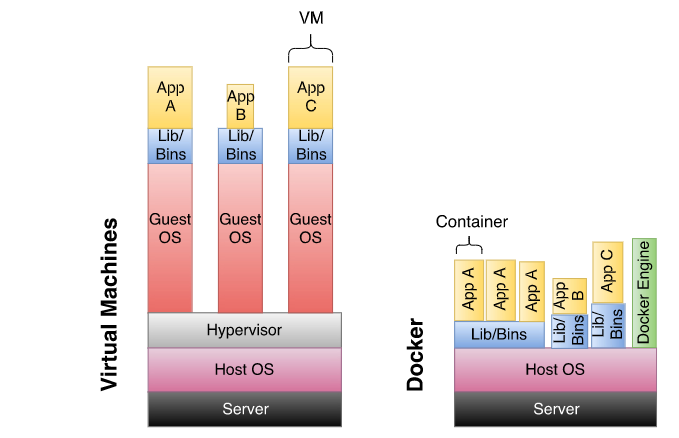
\includegraphics[width=\columnwidth]{gfx/vm vs container.png} %.5\textwidth
	\caption{Unterschied zwischen Virtualisierung und Container, Quelle: Albin Sundqvist \cite{sundqvist2020guidelines}}
\end{figure}

Abbildung 1 zeigt den Unterschied zwischen Virtualisierung und Containerisierung, wobei die Virtualisierung eine komplette Instanz eines Betriebssystems erfordert, während die Containerisierung lediglich die notwendigen Abhängigkeiten und Ressourcen für die spezifische Anwendung bereitstellt. Dies führt zu einer höheren Ressourceneffizienz und einer besseren Portabilität.

Ein weiterer Vorteil der Containerisierung ist die Möglichkeit, Legacy-Software in einem Container auszuführen, ohne dass die Notwendigkeit besteht, die Anwendung an die aktuelle Umgebung anzupassen.
Dies ermöglicht es Unternehmen, ältere Anwendungen weiterhin zu nutzen, ohne in die Wartung und Anpassung von Legacy-Code zu investieren.

\begin{description}
	\item[Beispiel einer Dockerfile:]\leavevmode
	\begin{lstlisting}
FROM openjdk:20-slim-buster
EXPOSE 8080
COPY target/demo-SNAPSHOT.JAR app.jar
ENTRYPOINT ["java","-jar","/app.jar"]
\end{lstlisting}
\end{description}


Obwohl die Containerisierung viele Vorteile bietet, wie die Verbesserung der Portabilität und Skalierbarkeit von Legacy-Software, gibt es auch Nachteile, die berücksichtigt werden müssen. Dazu gehören potenzielle Sicherheitsprobleme und die Notwendigkeit für die Erstellung und Wartung von Images. Es ist daher unerlässlich, die Vor- und Nachteile sorgfältig abzuwägen, bevor man sich für die Containerisierung einer Anwendung entscheidet.

In Bezug auf die Erstellung von Images, schaut Docker beim Erstellen eines Images zunächst in seinem Build-Cache nach, ob die benötigten Schichten bereits als Hash vorhanden sind und kann sie so wiederverwenden.


\textbf{Zusammengefasst:}
In der Informatik gibt es oft den Wunsch, Legacy-Software, also schwer veränderbare oder nicht verständliche Code, in Container zu verpacken, um die Portabilität und Skalierbarkeit zu verbessern.
Containerisierung ist eine Methode, um eine Laufzeitumgebung mittels Software zu virtualisieren. Dafür wird oft das Tool Docker verwendet, welches Container erstellen kann, die alle erforderlichen Abhängigkeiten enthalten, um die Software unabhängig auszuführen.
Im Gegensatz zu virtuellen Maschinen, die einen Hypervisor benötigen, laufen Container direkt auf dem Host-System. Container haben den Vorteil, dass sie nur die für die Software erforderlichen Abhängigkeiten besitzen und nicht den gesamten Overhead einer Virtualisierung. Images, die read-only Informationen enthalten, die für die Erstellung eines Containers erforderlich sind, werden in Schichten definiert und in einer Dockerfile definiert.
Diese Schichten können wiederverwendet werden und es wird ein Hashwert gezogen für den späteren Gebrauch.


\section{Szenario}
Im folgenden wird ein Szenario beschrieben, in dem Unternehmen Legacy-Software im Einsatz haben und die Problematiken, die sich daraus ergeben, dargestellt werden. Es wird gezeigt wie diese Problematiken mit Hilfe der Containerisierung gelöst werden können.

\subsection{Problematik}
Oftmals kann es vorkommen, dass Unternehmen Legacy-Software im Einsatz haben, die mehrere Jahre alt ist und teils nicht mehr gewartet wird oder nicht mehr mit den wachsenden Anforderungen Schritt hält. Diese Legacy-Software kann schnell zu einem Engpass in einem Workflow führen, insbesondere wenn es sich um eine systemkritische Komponente handelt. Das Ersetzen solcher Software kann je nach Umfang nur mit einem hohen Geldaufwand umgesetzt werden. Da die Software weder quelloffen ist noch einfach ausgetauscht werden kann, ist es sinnvoll sie zu containerisieren um sie anschließend zu skalieren. Dies wäre auch mittels virtuellen Maschinen möglich, jedoch ist zu beachten, dass dies einen erhöhten Konfigurationsaufwand hätte. Containerisierung ermöglicht es Unternehmen, ihre Legacy-Software weiterhin zu nutzen, ohne in die Wartung und Anpassung von Legacy-Code zu investieren und bietet die möglichkeit Anwendungen skalieren zu können, um den Anforderungen des Workflow gerecht zu werden.

\textbf{Zusammengefasst:}
In diesem Szenario geht es um Legacy-Software, die nicht mehr gewartet wird und nicht mehr mit den wachsenden Anforderungen Schritt hält. Diese Legacy-Software kann zu Engpässen in einem Workflow führen.
Es wird gezeigt, wie diese Problematiken mittels Containerisierung gelöst werden können, ohne in die Wartung und Anpassung von Legacy-Code zu investieren und Anwendungen skalieren zu können, um den Anforderungen des Workflows gerecht zu werden.
\section{Auftretende Probleme}

In diesem Kapitel werden die Herausforderungen bei der Containerisierung von Legacy-Software behandelt. Es werden diverse Probleme, die bei diesem Vorgang auftreten können, vorgestellt. Es werden die Aspekte des Source Codes, der Arbeitsweise der Software, der Installation und spezieller Abhängigkeiten untersucht, die bei der Containerisierung von Legacy-Software zu beachten sind. Es wird darauf eingegangen, welche Schwierigkeiten entstehen können und wie diese zu handhaben sind.

Die Containerisierung von Legacy-Software kann aufgrund ihrer Komplexität zu einer Herausforderung werden. Es gibt diverse Probleme, die auftreten und den gesamten Vorgang erschweren oder sogar unmöglich machen können. Um diese Probleme zu vermeiden, ist es wichtig, die folgenden Punkte sorgfältig zu prüfen, bevor man sich für die Containerisierung einer Anwendung entscheidet:

\subsection{Source Code:}
Legacy-Software kann der Source Code in den unterschiedlichsten Varianten vorliegen, manchmal auch gar nicht. Es gibt drei Möglichkeiten:
\subsubsection{}
Der Source Code ist vorliegend und man hat sogar die Möglichkeit, Änderungen vorzunehmen.
\subsubsection{}
Teilweise oder ganz vorliegend, aber keine Möglichkeit, Änderungen vorzunehmen.
\subsubsection{}
Der Source Code liegt nicht vor und ist somit weder änderbar noch einsehbar.

\subsection{Arbeitsweise der Software:}
Auch hier gibt es einige Punkte, die gegen eine Containerisierung sprechen, insbesondere Desktop-Anwendungen, die auf einem Frontend aufgebaut sind, das zu bedienen ist.
Der Mehraufwand, ein solches System in Betrieb zu nehmen, wäre höher als das Aufsetzen einer ganzen virtuellen Maschine.
Daher eignen sich eher Anwendungen, die Argumente über die Command Line annehmen und dann ohne weiteres Zutun ihre Arbeit verrichten.

\subsection{Installation:}
Hier gilt wie bei der Arbeitsweise der Software, dass eine Software nur mit einem erhöhten Mehraufwand installiert werden kann, wenn es dafür nur eine grafische Oberfläche gibt, die man bedienen muss.
Hierfür müssten dann alle Installationsschritte manuell (oder mittels Script) nachgestellt werden. Gerade bei einem Betriebssystem wie Windows kann dies zu einer äußerst mühseligen Arbeit werden.

\subsection{Spezielle Abhängigkeiten:}
Je nach Software kann es sein, dass spezielle Abhängigkeiten vorhanden sind, wie z.B.  Lizenzen. Dies ist oft der Fall, wenn die Software eingekauft wurde.
Diese können oder müssen entsprechend in den Container integriert werden.
Es kann auch vorkommen, dass Hardware-Abhängigkeiten bestehen, wie z.B. Lizenzen, die nur für bestimmte Hardware-Konfigurationen, Mac-Adressen oder ähnliches erstellt wurden und nur für diesen Computer freigegeben sind.
Dies sind besonders schwierige Fälle, für die es aber auch Lösungsansätze gibt.

\subsection{Speichern von Daten:}
Oftmals verarbeiten Programme Daten, die auf externen Datenträgern gespeichert werden.
Dies kann bei der Containerisierung von Legacy-Software zu Problemen führen, da die Daten nicht immer einfach zugänglich oder migrierbar sind.
Hier ist es wichtig, sicherzustellen, dass die Daten zugänglich und migrierbar sind, bevor man sich für die Containerisierung entscheidet.

\subsection{Uvm...}
Aufgrund der komplexität dessen werde ich nur ein paar Lösungsansätze für die oben beschrieben probleme angehen und eine der Lösungen vorstellen.

\textbf{Zusammengefasst:}

Im Kapitel III wurden die Herausforderungen bei der Containerisierung von Legacy-Software behandelt. Es wurden diverse Probleme vorgestellt, die bei diesem Vorgang auftreten können, wie z.B. die Aspekte des Source Codes, der Arbeitsweise der Software, der Installation und spezieller Abhängigkeiten. Es wurde erläutert, welche Schwierigkeiten entstehen können und wie diese zu handhaben sind.

\section{Lösungsansätze}
Im vierten Kapitel werden Lösungsansätze für die Herausforderungen bei der Containerisierung von Legacy-Software behandelt. Dabei werden die Aspekte des Source Codes, der Arbeitsweise der Software, der Installation und spezieller Abhängigkeiten, die bei der Containerisierung von Legacy-Software zu beachten sind, genauer untersucht. Es wird auf mögliche Schwierigkeiten eingegangen und gezeigt, wie diese zu handhaben sind. Es werden Lösungsansätze für die verschiedenen Probleme aufgezeigt, die bei der Containerisierung von Legacy-Software auftreten können.
\subsection{Source Code:}
Hier werden die verschiedenen Möglichkeiten der Verfügbarkeit des Source Codes von Legacy-Software und die damit verbundenen Herausforderungen bei der Containerisierung behandelt.
Es wird untersucht, wie man das Verhalten der Software verstehen und den Container entsprechend anpassen kann.
\subsubsection{Quelloffen}
Dies ist sehr unproblematisch, man kann das Verhalten der Software nachvollziehen und ggf. sogar ändern.

\subsubsection{Nicht quelloffen aber dokumentiert:}
Hier lassen sich zwar keine Änderungen vornehmen, aber man kann entsprechend der Dokumentationsqualität das Verhalten nachvollziehen und sich darauf entsprechend einstellen bzw. den Container entsprechend anpassen.

\subsubsection{Nicht quelloffen und nicht dokumentiert:}
Da weder Sourcecode noch Dokumentation vorhanden, gibt es hier leider nur zwei Möglichkeiten.
Den Hersteller zu Rate ziehen oder durch Try and Error oder gar durch Reverse Engineering \cite{eilam2011reversing} (Achtung: kann strafrechtliche Folgen mit sich ziehen siehe \cite{Richtlinie}) das Verhalten des Programms zu ergründen.

ganze einmal umformatieren mit subsections und subsubsection, dann nach jeden kaptel einmal eine kleiner zusammenfassung des selbigen, unter jeder section die leute mal bischen mitnehmen und kurz beschreiben was jetzt kommt.

\subsection{Arbeitsweise der Software:}
Wie bereits im Unterpunkt \textbf{Auftretende Probleme} beschrieben, macht es natürlich wenig Sinn, Software zu containerisieren, die trotzdem noch handisch bedient werden muss.
Dies ist auch ein klarer Ausschlusspunkt für die Containerisierung, da immer noch Personal benötigt wird, um es zu bedienen und der Mehraufwand dies zu bewerkstelligen höher als der Nutzen wäre.
Dennoch möchte ich hier kurz eine Möglichkeit aufzeigen. Software, die ein Webfrontend besitzt, kann man nicht nur prima containerisieren, sondern auch mittels Puppeteer vollautomatisch bedienen lassen.

\subsection{Installation:}
Auch hier ist es äußerst problematisch, wenn Software über eine Installationsroutine verfügt, durch die man sich durch Klicken muss.
Gerade im Windows-Umfeld erlebt man dies sehr häufig. Abhilfe dafür gibt es, gerade auch für Windows-Software, in Form der Installation via Command Line Interface.
Für die \textbf{Windows Microsoft Standard Installer} (in kurz MSI-Files) gibt es folgende Websites, die man zu Rate ziehen kann: \textbf{Microsoft Standard Installer Command-Line Optionen} \cite{microsoft} oder die folgende Seite, die nicht nur Microsoft-bezogen ist: \textbf{Silent Install HQ} \cite{silent}, die einem mit genug Tutorials versorgt, um die entsprechende Software dann doch zu installieren.

\subsection{Spezielle Abhängigkeiten}
Lizenzen müssen in die entsprechenden Container integriert werden. Handelt es sich hier um simple Lizensdateien, kann man diese via \textbf{COPY} oder \textbf{ADD} in der Dockerfile hinzufügen.
Schwieriger wird es hingegen, wenn wirklich Hardware-Abhängigkeiten bestehen. Zwar lassen sich Docker-Container hier vielfältig anpassen, z.B die Mac- oder IP-Adresse, aber auch hier gibt es gewisse Beschränkungen, da ein Container nicht endlos anpassbar ist.
Sollten hier Probleme aufgrund eines gesonderten Authentisierungsverfahrens auftreten, sollte man den Hersteller zu Rate ziehen. In diesem Fall kann es sinnvoll sein, spezielle Hardware-Abhängigkeiten in einer virtuellen Maschine zu emulieren, anstatt sie direkt in den Container zu integrieren.
Dies erfordert jedoch eine gründliche Analyse und Planung, um sicherzustellen, dass die Emulation korrekt funktioniert und die Performance nicht beeinträchtigt wird.
Eine weitere Möglichkeit besteht darin, eine spezielle Container-Plattform wie AWS Fargate oder Azure Container Instances zu verwenden, die spezielle Hardware-Unterstützung bereitstellen.

\subsection{Speichern von Daten:}
Da Container an sich zustandslos sind, wäre es äußerst unvorteilhaft, wenn alle Daten, die gespeichert werden müssen, nach einem Neustart verloren gingen.
Um dieses Problem zu lösen, hat Docker jedoch eine Lösung entwickelt. In der Dokumentation unter \textbf{Manage data in Docker} \cite{dockerrstorage} wird beschrieben, wie man nichtflüchtigen Speicher an Container anbinden kann. Diese Methode ermöglicht es, dass die gespeicherten Daten auch nach einem Neustart des Containers erhalten bleiben. Dieses Problem tritt natürlich nicht bei Containern auf, die nur Daten verarbeiten und dann weitergeben. Hier muss lediglich darauf geachtet werden, dass im Falle eines Absturzes die Arbeit am richtigen Punkt wieder aufgenommen wird. Es gibt mehrere Möglichkeiten um Daten in Containern zu speichern, man kann entweder eine Volume anlegen, welche auf dem Hostsystem liegen und von verschiedenen Containern gemountet werden können, oder man nutzt ein Volume-Management-Plugins, welches es ermöglicht, Datenbanken oder ähnliches in einem eigenen Volume zu speichern. Es ist wichtig vor der Verwendung von Containern sorgfältig die Anforderungen an den Datenspeicher zu prüfen und die passende Lösung für das Projekt zu wählen.

\textbf{Zusammengefasst:}
In Kapitel IV wurden Lösungsansätze für die Herausforderungen bei der Containerisierung von Legacy-Software behandelt. Es wurden die Aspekte des Source Codes, der Arbeitsweise der Software, der Installation und spezieller Abhängigkeiten genauer untersucht und Lösungsansätze für die möglichen Probleme aufgezeigt. Für den Fall, dass der Source Code nicht verfügbar ist, wurden verschiedene Möglichkeiten wie das Verhalten der Software zu verstehen und den Container anzupassen besprochen, wie z.B. den Hersteller um Rat zu fragen oder Reverse Engineering zu nutzen. Es wurde auch gezeigt, dass es für bestimmte Arten von Software, die noch manuell bedient werden müssen, keinen Sinn macht diese zu containerisieren. Eine Lösung für dieses Problem wäre die Verwendung von Software mit Webfrontend und die Nutzung von Puppeteer zur automatischen Bedienung.

\section{Zusammenfassung und Ausblick}

Die Containerisierung von Legacy-Software stellt eine große Herausforderung dar, da diese oft als historisch gewachsene Anwendungen oder Altlasten betrachtet werden. Dies kann vorkommen, wenn die Software aus Kostengründen eingekauft wird, die nicht quelloffen ist und im Laufe der Zeit nicht an die eigenen Anforderungen angepasst wird. Eine Möglichkeit, Legacy-Software zu modernisieren und für eine bessere Portabilität und Skalierbarkeit fit zu machen, ist die Containerisierung.

Containerisierung ist eine Technologie, die dazu verwendet wird, die Virtualisierung einer Laufzeitumgebung mittels Software zu gewährleisten. Ein gängiges Tool zur Containerisierung ist Docker, das Container erstellen kann, die alle notwendigen Abhängigkeiten besitzen, um Software unabhängig auszuführen. Der Vorteil von Containern ist, dass sie so konfiguriert werden können, dass sie nur die für die Software erforderlichen Abhängigkeiten besitzen und nicht den gesamten Overhead einer Virtualisierung.

In dieser Arbeit wird aufgezeigt, welche Anforderungen an die zu containerisierende Software bestehen und welche Probleme und Einschränkungen innerhalb eines Windows-Umfelds auftreten können. Es wird gezeigt, dass die Containerisierung von Legacy-Software eine Herausforderung darstellt, insbesondere in Bezug auf die Anpassung an die Anforderungen des Host-Systems und die Behandlung von Abhängigkeiten. Es wird auch diskutiert, wie die Erstellung von Images für Container durchgeführt wird und wie die Verwendung von Dockerfiles dazu beitragen kann, den Prozess der Containerisierung zu vereinfachen.

Insgesamt zeigt diese Arbeit, dass die Containerisierung von Legacy-Software eine Herausforderung darstellt, aber durch den Einsatz von Tools wie Docker und durch die Berücksichtigung bestimmter Anforderungen und Einschränkungen erfolgreich durchgeführt werden kann. Es wird empfohlen, die Containerisierung von Legacy-Software sorgfältig zu planen und durchzuführen, um die Vorteile von besserer Portabilität und Skalierbarkeit zu nutzen, ohne dabei die Funktionsfähigkeit der Software zu beeinträchtigen. Weiterhin ist es wichtig, die Anforderungen an die containerisierte Legacy-Software genau zu definieren und sicherzustellen, dass die Containerumgebung alle notwendigen Ressourcen und Abhängigkeiten bereitstellt, damit die Software ordnungsgemäß funktioniert. Es ist auch wichtig, die Sicherheitsaspekte der containerisierten Legacy-Software zu berücksichtigen und sicherzustellen, dass sie auf dem neuesten Stand der Technik sind. Ein weiteren wichtiger Aspekt ist die Handhabung von Daten in Containern, da diese an sich zustandslos sind und alle Daten, die gespeichert werden müssen, nach einem Neustart verloren gehen können. Docker bietet hierfür jedoch Lösungen wie das Anbinden von nicht-flüchtigem Speicher an Container, die in der Dokumentation unter "Manage data in Docker" beschrieben werden. Insgesamt erfordert die Containerisierung von Legacy-Software eine gründliche Planung und Durchführung, um die Vorteile der Portabilität und Skalierbarkeit zu nutzen, ohne die Funktionsfähigkeit der Software zu beeinträchtigen.



% BIB
\bibliographystyle{IEEEtran}
% argument is your BibTeX string definitions and bibliography database(s)
\bibliography{IEEEexample}

% that's all folks
\end{document}

